\section{Model-Based Testing}

Model-based testing is a software testing technique that uses test generation algorithms and a behavioral model of the system under test to generate test cases~\cite{1200168}. Unlike traditional development techniques which tend to focus on implementation, model-driven software development
stresses the use of models at all levels of the software
development process~\cite{5381477}. Like the data-driven and keyword-driven approaches to testing, model-based testing relies heavily on abstraction. However, the definition of a model varies greatly, depending on the approach~\cite{Jääskeläinen2008}. Instead of writing hundreds of test cases the test designer writes an abstract model of the system under test, and then the model-based testing tool generates a set of test cases from that same model. It allow to easily generate a large test suite from the same model or regenerate the test suite each time the system requirements change. By following this approach, the test design time is reduced and several test suites can be generated by just using different test criteria. The purpose of model-based testing is to solve problems~\cite{1200168} that other testing processes do not fully address like:
\begin{itemize}
\item Automation of the design of functional test cases to reduce the design cost;
\item Produce test suites with systematic coverage of the model;
\item Reduction of the maintenance costs of the test suite;
\item Automatic generation of the traceability matrix from requirements to test cases.
\end{itemize}

\begin{figure}[!ht]
\centering
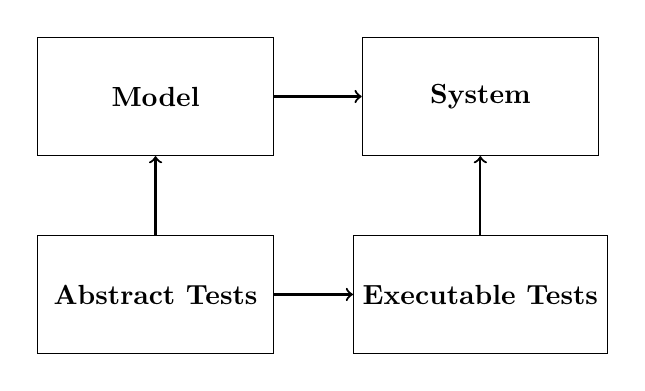
\begin{tikzpicture}
\matrix [column sep=10mm, row sep=10mm] {
  \node (model) [draw, shape=rectangle, minimum width=3cm, minimum height=1.5cm] {\textbf{Model}}; & \node (system) [draw, shape=rectangle, minimum width=3cm, minimum height=1.5cm] {\textbf{System}}; \\
  \node (abstests) [draw, shape=rectangle, minimum width=3cm, minimum height=1.5cm] {\textbf{Abstract Tests}}; & \node (exectests) [draw, shape=rectangle, minimum width=3cm, minimum height=1.5cm] {\textbf{Executable Tests}}; \\
};
\draw[->, thick] (abstests) -- (model);
\draw[->, thick] (exectests) -- (system);
\draw[->, thick] (model) -- ([yshift=-5mm]system);
\draw[->, thick] (abstests) -- ([yshift=-10mm]exectests);
\end{tikzpicture}
\caption{Model-driven definition} \label{fig:f3}
\end{figure}

Summing up, the model is a partial description of the system under test, the abstract tests are derived from the model, and the executable tests are the concrete implementation of the abstract tests that can be run against the system under test.

%\noindent This approach is increasingly gaining the attention of
%both industry and academia. Actually, is considered as 
%leading-edge technology in industry. Unlike traditional
%development techniques which tend to focus on
%implementation, model-driven software development
%stresses the use of models at all levels of the software
%development process~\cite{5381477}.

\subsection{How to model a system?}

The first and most important step in modeling a system for testing is deciding the level of abstraction of the model. It should be clear which aspects of the system under test to include in the model and which aspects to omit. We should always have in mind that a smaller model is often more useful than a large and complex model, since it allow us to test each one of them independently and think about which operations should be included before writing a model for the whole system. 

When modeling a system is also important to think about the data that it manages, the operations that it performs, and the subsystems that it communicates with. The difficulty of test generation is usually highly dependent on the number and range of the input parameters, so applying the same abstraction principle~\cite{Mosley2002} to its input and output parameters helps to control the test generation effort.

% TODO: Define the modeling notation!
After the test generation from the model and the execution of those tests against the system, each test that fails will point either to an error in the implementation of the system or to a mistake in the model. The value of model-based testing comes from the automated cross-checking between the model and the system implementation.
 
\subsection{Challenges in Modeling}
Model-based testing can improve considerably the test 
efficiency and test quality when the models are light 
and available. The elaboration of a model is, probably, 
the key for the success of model-based testing in practice,
and if done wrongly~\cite{Peleska.2013} can lead to a set of undesirable 
outcomes:

\begin{itemize}
\item If complex models have to be completed before testing
can start, this induces an unacceptable delay for the
proper test executions;
\item For complex SUT, like systems of systems, test models 
need to abstract from a large amount of detail, because 
otherwise the resulting test model would become unmanageable;
\item The required skills for test engineers writing test 
models are significantly higher than for test engineers 
writing sequential test procedures.
\end{itemize}

\subsection{Prerequisites of model-based testing}

It is important to have some high-level management support for the adoption of model-based testing, as well as some enthusiasm for model-based testing among the team who will put it into practice.

Model-based testing tools implies that the test execution phase is already automated. So, for a testing team who has little experience with automated testing might be wise to gain experience with an automated approach like data or keyword-driven testing before using model-based testing.

Model-based testing models are more precise than most UML models and require detailed modeling of the system behavior. Developing these kinds of models is more similar to programming than to designing use cases and class diagrams. It is helpful to have some experience with designing interfaces and choosing good levels of abstraction.

Sometimes, model-based testing does not suit the system needs. If the system has to be tested manually because the test steps require human interaction, then the cost of that manual testing may dominate any cost savings of model-based testing.

\subsection{Model-Based Testing and Agile methods}

%TODO
In addition, in terms of industrial adoption, MBT needs to be adapted to the existing testing processes that are shifting towards more agile practices [14] from the traditional ones based on the V-model [15] and its variations. In agile contexts, on the one hand, developers are already relying on test automation to support refactoring and generally understand its benefits as compared to manual testing. 

In the eyes of the agile practitioners, writing acceptance tests
that specify what the system is supposed to do, brings lot of value:
\begin{itemize}
\item It forces the customer to specify precisely what is required;
\item When the acceptance tests are “green” the customer has much 
more confidence that real and useful work has been done;
\item An executable specification gives a clear and measurable 
objective to the development team.
\end{itemize}

Having the acceptance tests centered around a model it makes 
not only easier to develop a significant number of acceptance tests,
but also to change the model and regenerate those same tests.

We can benefit even more from mixing model-based and acceptance tests, if the model itself is built around some agile principles:
\begin{itemize}
\item Test models should have a precise purpose;
\item Test models should be light; 
\item Test models should grow incrementally through an iterative approach;
\item Test models encourage discussion about the exact behavior of the system;
\item Test models should not be used for documentation.
\end{itemize}

\subsection{Advantages of model-based testing}
Model-based testing can lead to less time and effort spent
on testing if the time needed to write and maintain the model 
plus the time spent on directing the test generation is less 
than the cost of manually designing and maintaining a test suite. The use of an automated test case generator based on algorithms and heuristics to choose the test cases from the model makes the design process systematic and repeatable.

%TODO
 on the time costs of testing, showing that model-based testing can have a small cost-benefit over keyword-based testing and a significant cost-benefit over the other test- ing processes. 

%TODO
 it is very easy to generate more tests; with the push of another button or a few minutes choosing some more test selection criteria,

%TODO
As well as the quantity of tests, the quality of the test suite is also very important, and several studies have shown that the use of a model tends to increase fault detection effectiveness [DJK+99, FHP02, PPW+05].

%TODO
The other major benefit comes from the modeling stage—it is usual to find numerous “issues” (faults) in the requirements and design documents as a side-effect of modeling. The detection of such faults at an early stage can be a major benefit of model-based testing.

In spite of all of these benefits, the industrial adoption of this technology has been slow.

Robinson [3] states that the most common problems in deployment are the managerial difficulties, the making of easy-to-use tools, and the reorganization of the work with the tools. Hartman [4] reports problems with the complexity of the provided solution and counter-intuitive modeling. Our early experiences support these findings. Moreover, it must be acknowledged that modeling needs a special kind of expertise that may not be available in a testing organization. 

\subsection{Disadvantages of model-based testing}
One of the fundamental limitations of model-based testing is that it cannot guarantee to find all the differences between the model and the implementation, not even if there are hundreds of test cases being generated by the system model.

Model-based testing is not as trivial as other testing techniques, and requires a steep learning curve and different testing skills: modeling and programming skills. It is desirable to have a reasonably mature testing process and some experience with automated test execution before fully adopt this approach.

Up to date requirements plays a big role in model-based testing. The test cases are very coupled to the requirements, and requirements change, often. If the model is build based on outdated requirements, it will lead to unreliable results.

When one of these tests fails, it's hard to check if the failure is caused by the system under test, the driver, or even from the model itself. This process makes more difficult and time-consuming to find the root cause of the failing test.

Since this approach can generate huge numbers of tests, it becomes necessary to move toward other measurements of test progress instead of relying on the number-of-tests metric. Business code, requirements and model coverage are some of the alternatives.

